%%%%%%%%%%%%%%%%%%%%%%%%%%%%%%%%%%%%%%%%%
% Journal Article
% LaTeX Template
% Version 1.3 (9/9/13)
%
% This template has been downloaded from:
% http://www.LaTeXTemplates.com
%
% Original author:
% Frits Wenneker (http://www.howtotex.com)
%
% License:
% CC BY-NC-SA 3.0 (http://creativecommons.org/licenses/by-nc-sa/3.0/)
%
%%%%%%%%%%%%%%%%%%%%%%%%%%%%%%%%%%%%%%%%%

%----------------------------------------------------------------------------------------
%	PACKAGES AND OTHER DOCUMENT CONFIGURATIONS
%----------------------------------------------------------------------------------------

\documentclass[twoside]{article}

\usepackage{lipsum} % Package to generate dummy text throughout this template
%\usepackage[caption=false]{subfig}
%\captionsetup[subfigure]{labelformat=brace}
\usepackage{graphicx, bm} % Required to insert images
\usepackage{capt-of}%%To get the caption
\usepackage{listings} % Required for insertion of code
\usepackage[usenames,dvipsnames]{color} % Required for custom colors
\usepackage[sc]{mathpazo} % Use the Palatino font
\usepackage[T1]{fontenc} % Use 8-bit encoding that has 256 glyphs
\linespread{1.05} % Line spacing - Palatino needs more space between lines
\usepackage{microtype} % Slightly tweak font spacing for aesthetics

\usepackage{amsmath}
\usepackage{amssymb}

\usepackage[hmarginratio=1:1,top=32mm,columnsep=20pt]{geometry} % Document margins
\usepackage{multicol} % Used for the two-column layout of the document
\usepackage[hang, small,labelfont=bf,up,textfont=it,up]{caption} % Custom captions under/above floats in tables or figures
\usepackage{booktabs} % Horizontal rules in tables
\usepackage{float} % Required for tables and figures in the multi-column environment - they need to be placed in specific locations with the [H] (e.g. \begin{table}[H])
\usepackage{hyperref} % For hyperlinks in the PDF

\usepackage{lettrine} % The lettrine is the first enlarged letter at the beginning of the text
\usepackage{paralist} % Used for the compactitem environment which makes bullet points with less space between them
\usepackage{titlesec}


\usepackage{abstract} % Allows abstract customization
\renewcommand{\abstractnamefont}{\normalfont\bfseries} % Set the "Abstract" text to bold
\renewcommand{\abstracttextfont}{\normalfont\small\itshape} % Set the abstract itself to small italic text


\usepackage{fancyhdr} % Headers and footers
\pagestyle{fancy} % All pages have headers and footers
\fancyhead{} % Blank out the default header
\fancyfoot{} % Blank out the default footer
\fancyhead[C]{STAT-221: PSET 2 $\bullet$ October 2014} % Custom header text
\fancyfoot[RO,LE]{\thepage} % Custom footer text

%----------------------------------------------------------------------------------------
%	CODE INCLUSION CONFIGURATION
%----------------------------------------------------------------------------------------

\definecolor{MyDarkGreen}{rgb}{0.0,0.4,0.0} % This is the color used for comments
\lstloadlanguages{R} % Load Perl syntax for listings, for a list of other languages supported see: ftp://ftp.tex.ac.uk/tex-archive/macros/latex/contrib/listings/listings.pdf
\lstset{language=R, % Use Perl in this example
        frame=single, % Single frame around code
        basicstyle=\scriptsize\ttfamily, % Use small true type font
        keywordstyle=[1]\color{Blue}\bf, % Perl functions bold and blue
        keywordstyle=[2]\color{Purple}, % Perl function arguments purple
        keywordstyle=[3]\color{Blue}\underbar, % Custom functions underlined and blue
        identifierstyle=, % Nothing special about identifiers                                         
        commentstyle=\usefont{T1}{pcr}{m}{sl}\color{MyDarkGreen}\scriptsize, % Comments small dark green courier font
        stringstyle=\color{Purple}, % Strings are purple
        showstringspaces=false, % Don't put marks in string spaces
        tabsize=2, % 5 spaces per tab
        %
        % Put standard Perl functions not included in the default language here
        morekeywords={rand},
        %
        % Put Perl function parameters here
        morekeywords=[2]{on, off, interp},
        %
        % Put user defined functions here
        morekeywords=[3]{test},
       	%
        morecomment=[l][\color{Blue}]{...}, % Line continuation (...) like blue comment
        numbers=left, % Line numbers on left
        firstnumber=1, % Line numbers start with line 1
        numberstyle=\tiny\color{Blue}, % Line numbers are blue and small
        stepnumber=5 % Line numbers go in steps of 5
}

% Creates a new command to include a perl script, the first parameter is the filename of the script (without .pl), the second parameter is the caption
\newcommand{\Rscript}[2]{
\begin{itemize}
\item[]\lstinputlisting[caption=#2,label=#1]{#1.R}
\end{itemize}
}

%----------------------------------------------------------------------------------------
%	TITLE SECTION
%----------------------------------------------------------------------------------------

\title{\vspace{-15mm}\fontsize{24pt}{10pt}\selectfont\textbf{STAT-221: Pset 2}} % Article title

\author{
\large
\textsc{Kevin Kuate Fodouop}\\ % Your name
\normalsize Harvard University \\ % Your institution
%\normalsize \href{mailto:john@smith.com}{john@smith.com} % Your email address
\vspace{-5mm}
}
\date{}

%----------------------------------------------------------------------------------------

\begin{document}

\maketitle % Insert title

\thispagestyle{fancy} % All pages have headers and footers

%----------------------------------------------------------------------------------------
%	ABSTRACT
%----------------------------------------------------------------------------------------

\begin{abstract}
Large scale computation with clusters like Odyssey allows computation of Bayesian methods' frequency characteristics, like frequency coverage of Bayesian interval. In this problem set, we use MCMC samplling to evaluate such frequency properties for a non-conjugate hierarchical Bayesian model. A section is dedicated to each task (section number corresponds to task number).

\end{abstract}

%----------------------------------------------------------------------------------------
%	ARTICLE CONTENTS
%----------------------------------------------------------------------------------------

%\begin{multicols}{2} % Two-column layout throughout the main article text

\section{Model and Posterior Distribution}

We use the log-Normal/Poisson model, a non-conjugate hierarchical model. The data generating process for this model is:

\begin{align*}
p\left(\mu, \sigma^2\right) & \propto \frac{1}{\sigma^2}\\
log\left(\theta_j\right) & \sim N\left(\mu, \sigma^2\right), \quad \textit{j = 1, ..., J}\\
Y_{jn} & \sim Pois\left(w_j \* /theta_j\right), \quad \textit{j = 1, ..., J; n = 1, ..., N} 
\end{align*}
\begin{itemize}
\item $\mu$ and $\sigma^2$ unknown constants, hyperparameters of the model.
\item $\theta_j$ latent variables, basic intensity of unit $j$, drawn from a distribution common to each unit.
\item $w_j$ known constant, exposure weight for unit $j$.
\item $Y_{j, n}$ random variables, set of N Poisson observations drawn for each unit.
\end{itemize}
\vspace{.2 in}
We derive the joint posterior for $\mu$, $\sigma^2$, $\log\left(\vec{\theta}\right)$ for our model:
\begin{align*}
P\left[\mu, \sigma^2, log\left(\vec{\theta}\right) | Y\right] & \propto	P\left[Y | \mu, \sigma^2, log\left(\vec{\theta}\right)\right] \times P\left[\mu, \sigma^2, log\left(\vec{\theta}\right)\right]\\
& = P\left[Y | \mu, \sigma^2, log\left(\vec{\theta}\right)\right] \times P\left[log\left(\vec{\theta}\right) | \mu, \sigma^2 \right] \times P\left[\mu, \sigma^2\right]\\
& \propto \prod_{j=1}^J \prod_{n=1}^N \frac{(w_j \theta_j)^{y_{jn}}}{y_{jn}!} \* e^{-w_j \* \theta_j} \times \prod_{j=1}^J \frac{1}{ \sigma} \* e^{ - \frac{\left(log\left(\theta_j\right) - \mu\right)^2}{2 \* \sigma^2}} \times \frac{1}{\sigma^2}\\
& = \frac{1}{\sigma^{J + 2}} \* e^{- \sum_{j=1}^J \frac{\left(log\left(\theta_j\right) - \mu\right)^2}{2 \* \sigma^2}} \* \prod_{j=1}^J \prod_{n=1}^N \frac{(w_j \theta_j)^{y_{jn}}}{y_{jn}!} \* e^{-w_j \* \theta_j}\\
& \propto \frac{1}{\sigma^{J + 2}} \* e^{- \sum_{j=1}^J \frac{\left(log\left(\theta_j\right) - \mu\right)^2}{2 \* \sigma^2}} \* \prod_{j=1}^J \prod_{n=1}^N \theta_j^{y_{jn}} \* e^{-w_j \* \theta_j} \quad (1)
\end{align*}
And the the conditional posterior of $log\left(\theta_j\right)$ is given by ($\vec{w}$ is not included in the conditioning, as supposed known) normalizing (1)'s component corresponding to unit $j$ by $(\mu, \sigma^2)$'s posterior probability:
\begin{align*}
P\left[log\left(\theta_j\right) | \mu, \sigma^2, Y\right] & =  \frac{P\left[\mu, \sigma^2, log\left(\theta_j\right) | Y\right]}{P\left[\mu, \sigma^2 | Y\right]}\\
& \propto P\left[\mu, \sigma^2, log\left(\theta_j\right) | Y\right]\\
& \propto  \* e^{- \frac{\left(log\left(\theta_j\right) - \mu\right)^2}{2 \* \sigma^2}} \* \theta_j^{S_j} \* e^{- n \* w_j \* \theta_j}
\end{align*}
with $S_j = \sum_{n=1}^N y_{jn}$.\\
Denoting $z_j = log(\theta_j)$, the conditional posterior hence has a density
\begin{align*}
f_{post}(z_j) = e^{- \frac{\left(z_j - \mu\right)^2}{2 \* \sigma^2}} \* e^{S_j \* z_j} \* e^{- n \* w_j \* e^{z_j}}
\end{align*}
And a log-density
\begin{align*}
l_{post}(z_j) & = log \circ f_{post}(z_j)\\
&  = - \frac{\left(z_j - \mu\right)^2}{2 \* \sigma^2} + S_j \* z_j - n \* w_j \* e^{z_j}
\end{align*}
Which is concave as a sum of 3 concave (including 1 linear) functions. Hence \textbf{the conditional posterior is log-concave}.\\

Let's compute the derivatives of $l_{post}$:
\begin{align*}
\frac{\partial l_{post}}{\partial \d z_j} & = - \frac{z_j - \mu}{\sigma^2} + S_j - n \* w_j \* e^{z_j}\\
\frac{\partial^2 l_{post}}{\partial \d z_j^2} & = - \frac{1}{\sigma^2} - n \* w_j \* e^{z_j}
\end{align*}
$\frac{\partial^2 l_{post}}{\partial \d z_j^2} <0$, so $\frac{\partial l_{post}}{\partial \d z_j}$ is decreasing. Having $\frac{\partial l_{post}}{\partial \d z_j} \overset{-\infty}{\to} +\infty$ and $\frac{\partial l_{post}}{\partial \d z_j} \overset{+\infty}{\to} -\infty$, $\frac{\partial l_{post}}{\partial \d z_j}$ has one and only zero. So that the \textbf{conditional posterior of $log\left(\theta_j\right)$ is unimodal}.\\


-- To be removed --
We compute the denominator's probability by integrating $log\left(\vec{\theta}\right)$ out of (1):
\begin{align*}
P\left[\mu, \sigma^2 | Y \right] & \propto P\left[Y | \mu, \sigma^2 \right] \times P\left[\mu, \sigma^2\right]
\end{align*}
We obtain the first term by integrating $log\left(\vec{\theta}\right)$ out of the likelihood:
\begin{align*}
 P\left[Y | \mu, \sigma^2 \right] & = \int_{-\infty}^{+\infty} P\left[Y | \mu, \sigma^2, log\left(\vec{\theta}\right)\right] \* P\left[log\left(\vec{\theta}\right) | \mu, \sigma^2, \right]\,dlog(\vec{\theta})\\
 & \propto 
\end{align*}


-- --
%------------------------------------------------

\section{Linear Basis Function Regression}

We tried replication Bishop 1.4 plots of MLE weight vectors for 4 values of M, using both closed form expressions and gradient descent. The former gets very close agreement (figure 1).

\begingroup
\centering
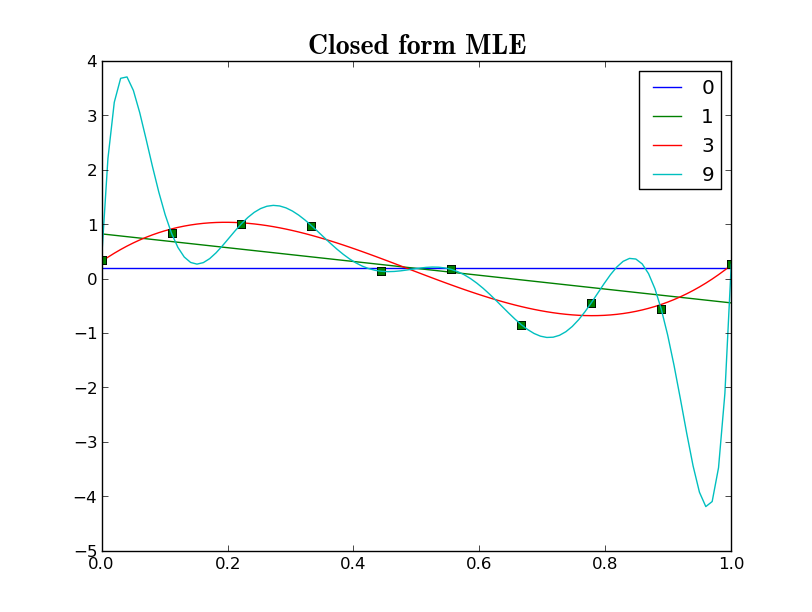
\includegraphics[scale=0.17]{./img/pol_reg_regfit.png}
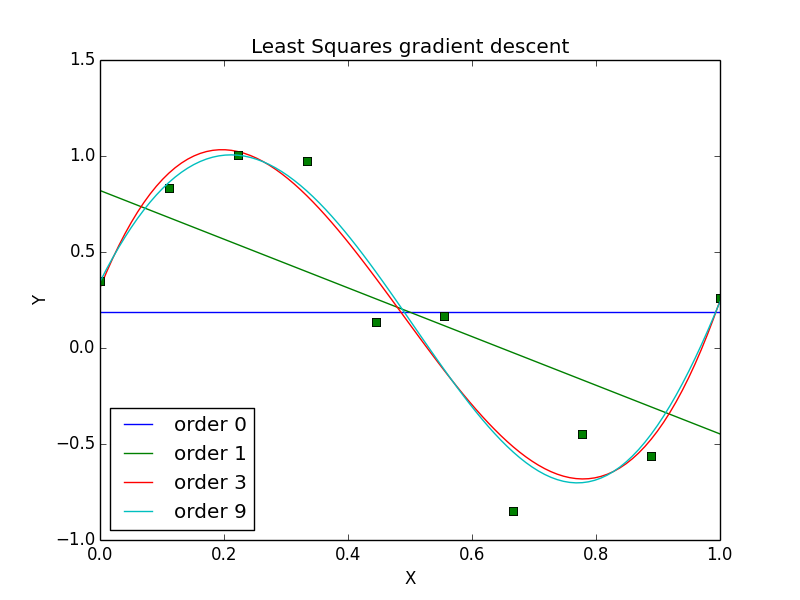
\includegraphics[scale=0.17]{./img/pol_grad_fit.png}
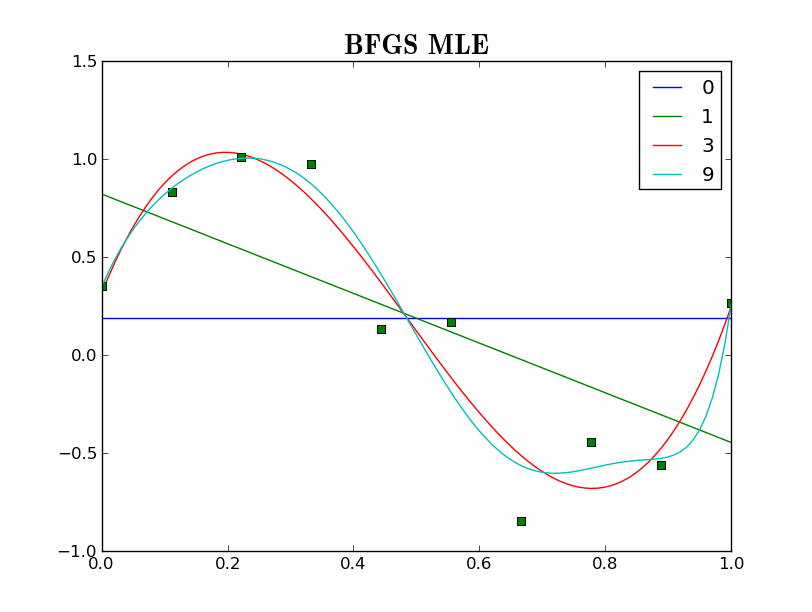
\includegraphics[scale=0.17]{./img/pol_bfgs_fit.png}
\captionof{figure}{MLE weight vector obtained using closed form expression (reproduces Bishop 1.4), using gradient descent and BFGS algorithm (optimize package), in order.}
\endgroup

The gradient descent and BFGS method uses the $SSE$ corresponding to current weight vector as objective function to minimize. Both optimization on the $SSE$ fails for too high orders. We think this is due to the optimized function having a plateau, from which the descent fails to progress towards the optimum.

%------------------------------------------------

\section{Ridge Regression}

\subsection{Ridge regression for Bishop's data}

Ridge regression regularizes coefficients for high polynomial orders, which were of in ranges up to $10^{15}$ for OLS. The cost function is cost$_{SSE}$ + $\lambda \sum_{i>0}w_i^2$\\
Plot obtained are more smooth and less likely to overfit. $\lambda=10^{-4}$ gives a pretty good fit for order superior to 3. $\lambda$ of $10^{-2}$ or more regularizes the weights too much, so that the fit for all orders is too flat to accurately fit the data.

\begingroup
\centering
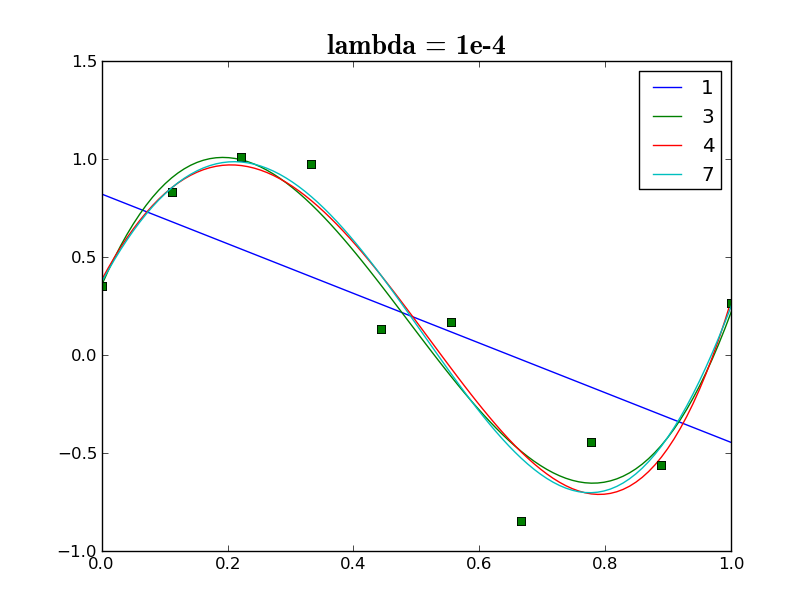
\includegraphics[scale=0.17]{./img/reg_1e4.png}
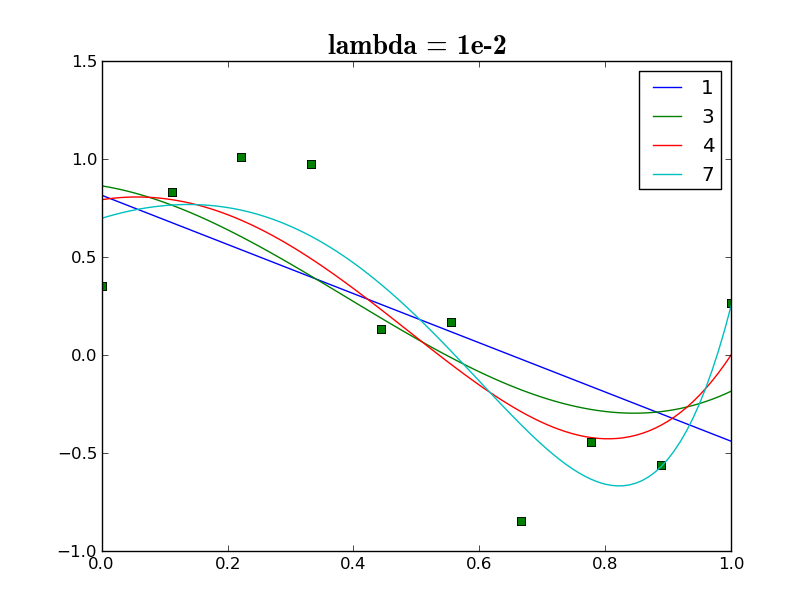
\includegraphics[scale=0.17]{./img/reg1e2.png}
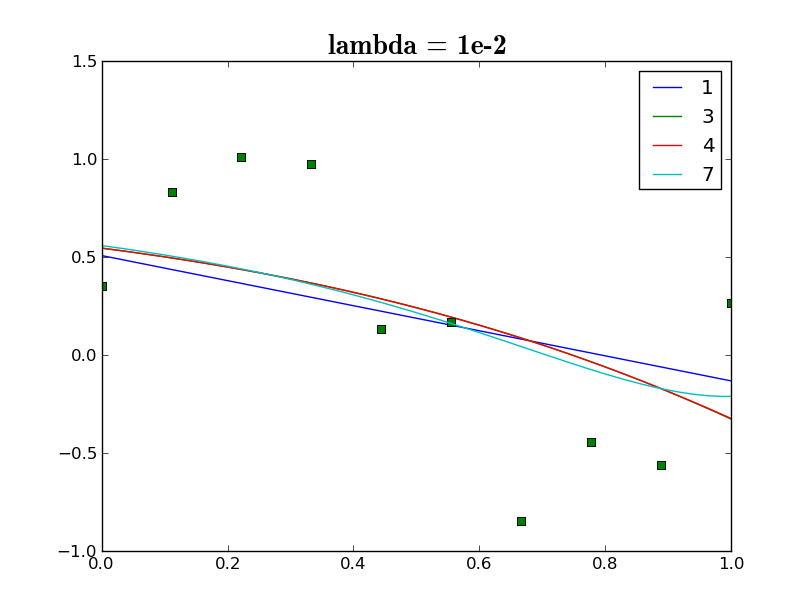
\includegraphics[scale=0.17]{./img/reg_1.png}
\captionof{figure}{Ridge regression fit for several values of M, for $\lambda \in [10^{-4}, 10^{-1}, 1]$ (in order).}
\endgroup

\subsection{Model selection with ridge regression}

We train ridge regressions for different $M$ and $\lambda$ on the two training sets A and B, $train_A$ and $train_B$. The \textit{validation data} is split in a validation set and a test set. SSE of models on the validation set is used to choose the best model originating from $train_A$ or $train_B$. Validation errors are compiled in table 2.\\

\begingroup
\centering
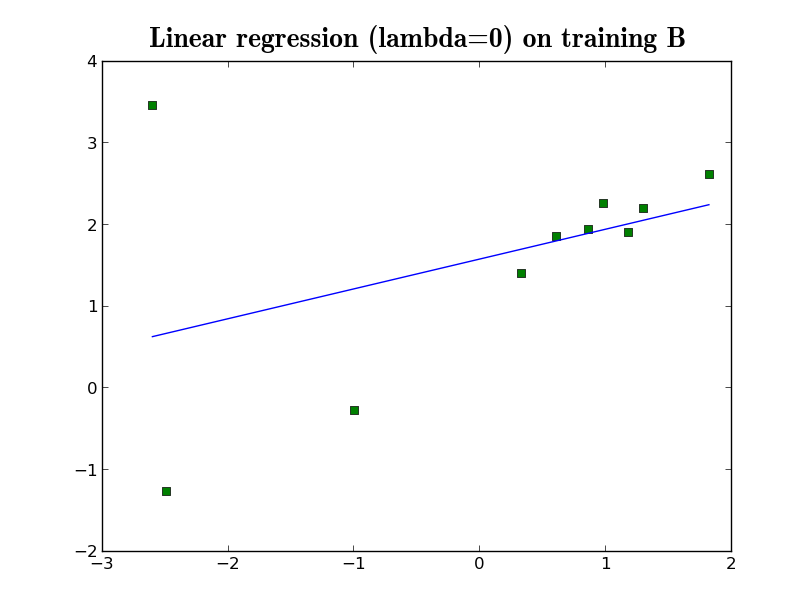
\includegraphics[scale=0.17]{./img/ridge_trainb_lin.png}
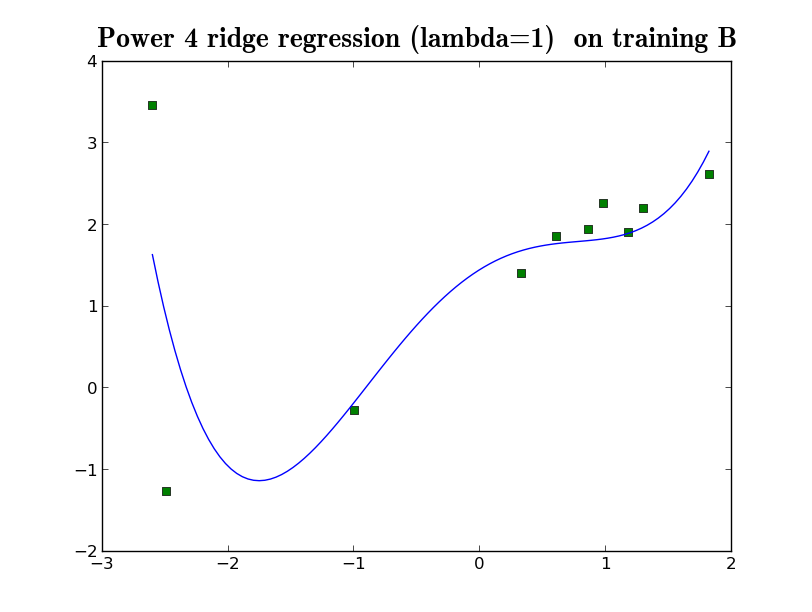
\includegraphics[scale=0.17]{./img/ridge_trainb_cub.png}
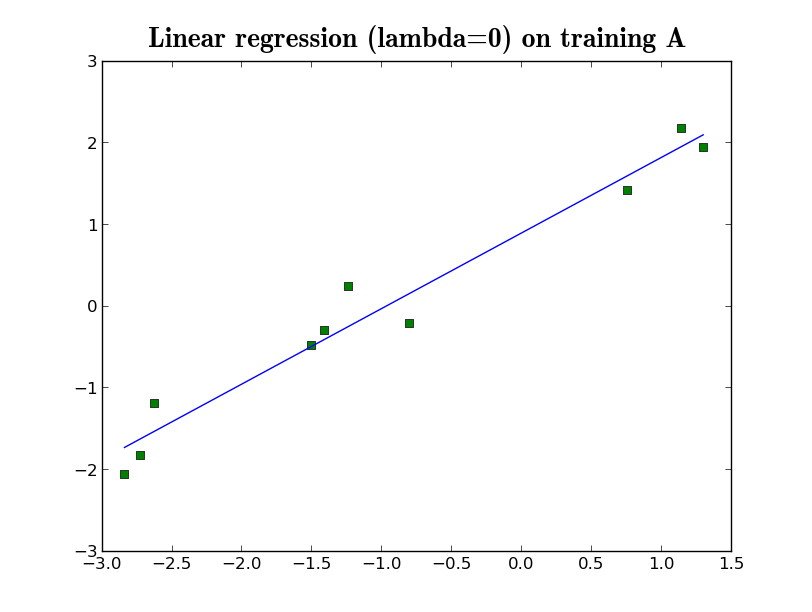
\includegraphics[scale=0.17]{./img/ridge_traina_lin.png}
\captionof{figure}{$train_A$'s data has a very linear shape, whereas an outlier in $train_B$ prevents the linear model from capturing the right correlation in data.} 
\endgroup


\begin{table}[H]
\caption{Some $(M, \lambda)$ combinations validation errors. Minimum SSE for each training set in blue.}
\centering
\begin{tabular}{llrr}
\toprule
Training set & M & $\lambda$ & $SSE_{val}$ \\
\midrule
A & 1 & 0 & \textcolor{blue}{0.73}\\
A & 3 & $10^{-1}$ &  1.6\\
A & 7 & $10$ & 88.7\\
B & 1 & $0$ & 16\\
B & 3 & $10^{-4}$ & 3.6\\
B & 4 & $1$ & \textcolor{blue}{0.41}\\
\bottomrule
\end{tabular}
\end{table}

We fitted ridge regression with $\lambda=10^{\pm i}, i=0...4$ and $\lambda=0$. The data in $train_B$ has a very linear form, so that no regularization is needed and regular linear regression is chosen. $train_B$ however has an outlier, which tampers the simple linear regression model (shifted up and lower slope). So that a well regularized ($\lambda = 1$) model of order 4 captures better the shape of the data, and obtains the best validation error.

When tried on the test set, the model issued from $train_A$ unsurprisingly performs better, with $SSE_{test}^{(A)} = 1.2$ compared to $SSE_{test}^{(B)} = 28$. Fit on test set plotted on figure 4.

\begingroup
\centering
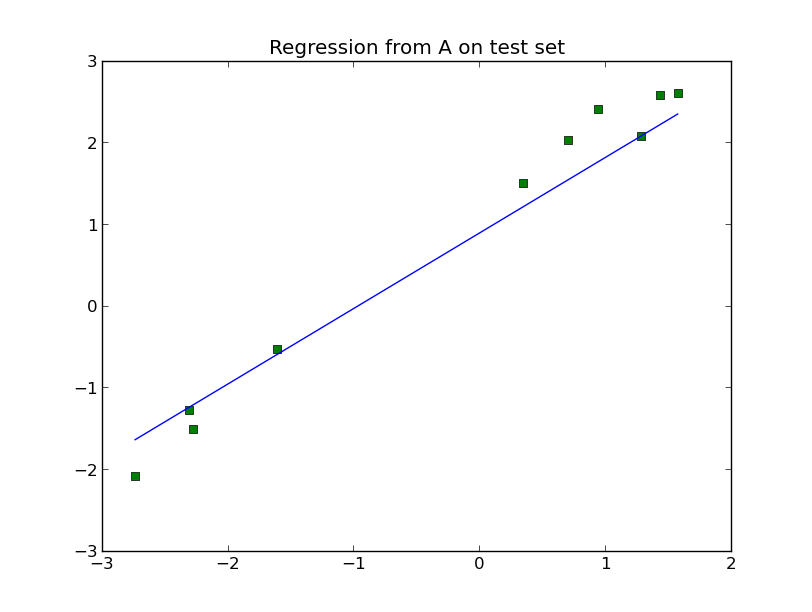
\includegraphics[scale=0.17]{./img/test_rega.png}
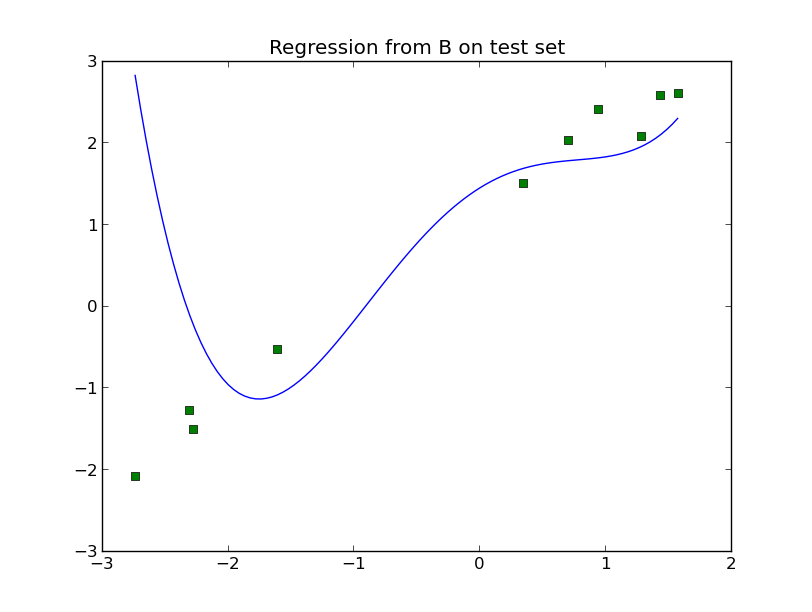
\includegraphics[scale=0.17]{./img/test_regb.png}
\captionof{figure}{Final models from $train_A$ and $train_B$'s fit on the test set.} 
\endgroup

\subsection{BlogFeedback data}
We perform a ridge regression on the BlogFeedback data set. We note that the design matrix $X$ is not full rank ($rank=246$ for 280 features), so that $X^T \* X$ is not invertible (some features are redundant). In consequence we use a pseudo-inverse function to compute the ridge regression.
\begin{table}[H]
\caption{Evolution of training error and validation error with $\lambda$ (optimal validation error in blue).}
\centering
\begin{tabular}{llr}
\toprule
$\lambda$ & $MSE_{train}$ & $MSE_val$\\
\midrule
$0$ & 881 & $4 \times 10^6$\\
$10^{-3}$ & 881 & $4 \times 10^6$\\
$10^{-1}$ & 881 &  $4 \times 10^6$\\
$10^{2}$ & 882 & $7 \times 10^5$\\
$10^{6}$ & 895 & $5 \times 10^5$\\
$10^{10}$ & 1209 & \textcolor{blue}{$1.5 \times 10^4$}\\
$10^{14}$ & 1372 & $3 \times 10^5$\\
\bottomrule
\end{tabular}
\end{table}

\begingroup
\centering
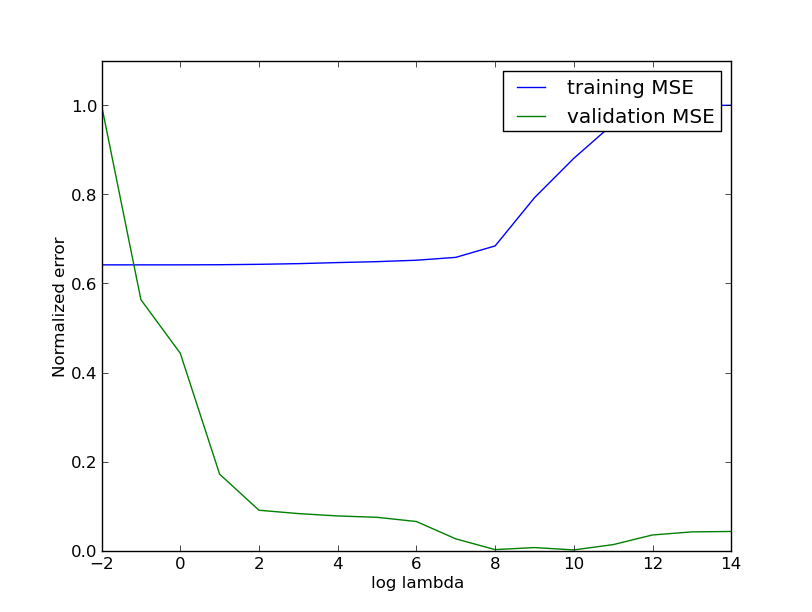
\includegraphics[scale=0.30]{./img/lambda_error.png}
\captionof{figure}{Training and validation $MSE$ plotted against $log_{10}(\lambda)$.} 
\endgroup
\vspace{0.2 in}
The OLS model suffers from overfitting due to the high number of variables. A high regularization coefficient is needed to obtain good validation error, and we find an optimal $\lambda=10^{10}$.\\
To find optimal $\lambda$, we started from small values ($10^{-4}$), assessed that increasing it led to better validation error, and increased it by ten-fold until an increase in validation error. Corresponding training and validation error are plotted on figure 5.\\
The selected model has an error on the test set $MSE_{selected}^{(test)} = 15 \times 10^{3}$, compared to $MSE_{OLS}^{(test)} = 4.5 \times 10^{6}$. Ridge weights are typically of an order of magnitude around $10^{-6}$ the ones of non-regularized weights.


%------------------------------------------------

\section{Generalizations}

We limit this part's study to order 5. Lower orders fit better the data (less overfitting) and benefit less from the regularization methods.

\subsection{Least absolute deviation}

Still using $train_A$ and $train_B$, we fit a \textit{least absolute deviations} (LAD) regression. We repeat our experiment of trying different regularizer weight $\lambda$, assess best fits on the validation error, and computes selected models fit on the test set. Sum of absolute errors (SAE) on the validation set are compiled for some $\lambda$ in table 4.

\begin{table}[H]
\caption{Some $(M, \lambda)$ combinations validation errors for LAD ($order = 5$). Minimum SAE for each training set in blue.}
\centering
\begin{tabular}{llrr}
\toprule
Training set & $\lambda$ & $SAE_{val}$ \\
\midrule

A & $10^{-4}$ &  5.8\\
A & $10^{-1}$ & \textcolor{blue}{5.7}\\
A & $10^3$ & 11\\
B & $10^{-3}$ & 24\\
B & $10$ & \textcolor{blue}{14}\\
B & $10^2$ & 16\\
\bottomrule
\end{tabular}
\end{table}

\begingroup
\centering
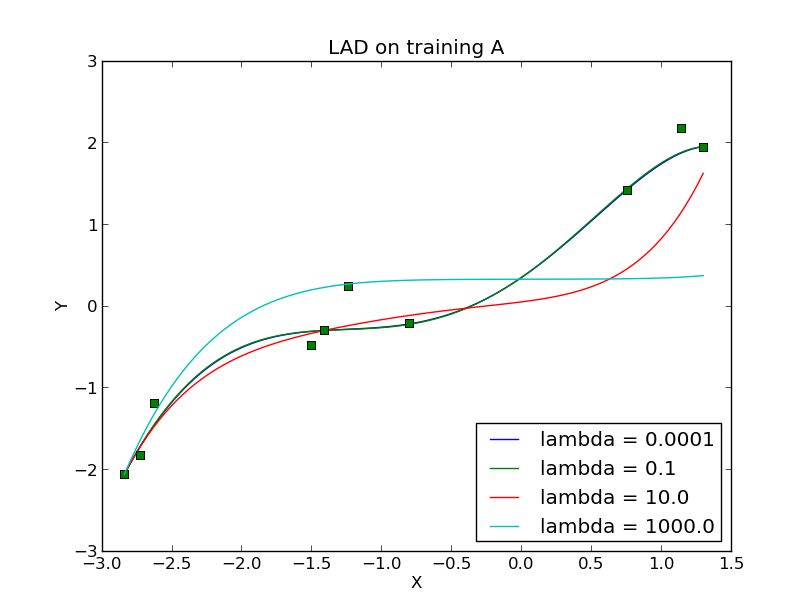
\includegraphics[scale=0.17]{./img/LAD.png}
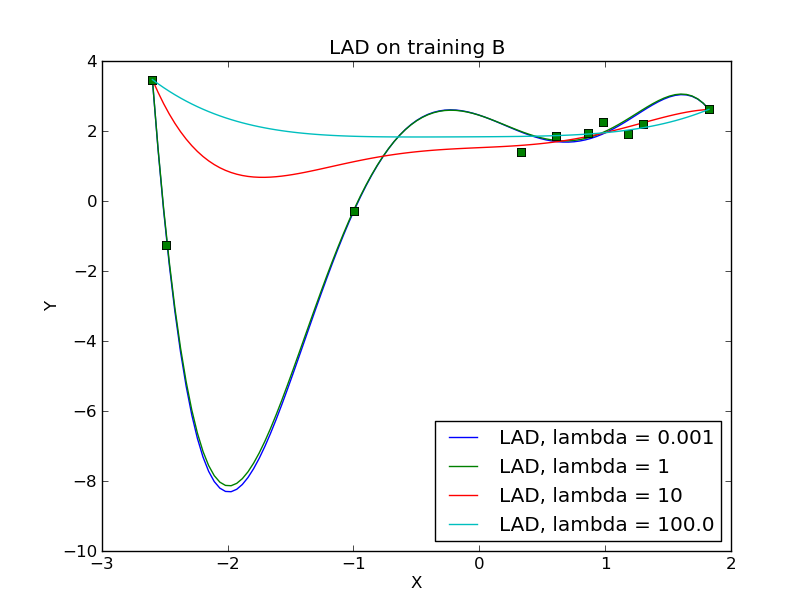
\includegraphics[scale=0.17]{./img/LAD_B.png}
\captionof{figure}{Training fit for LAD ($order=5$) with different $\lambda$ for $train_A$ (left) and $train_B$ (right).} 
\endgroup
\vspace{0.2 in}

\begingroup
\centering
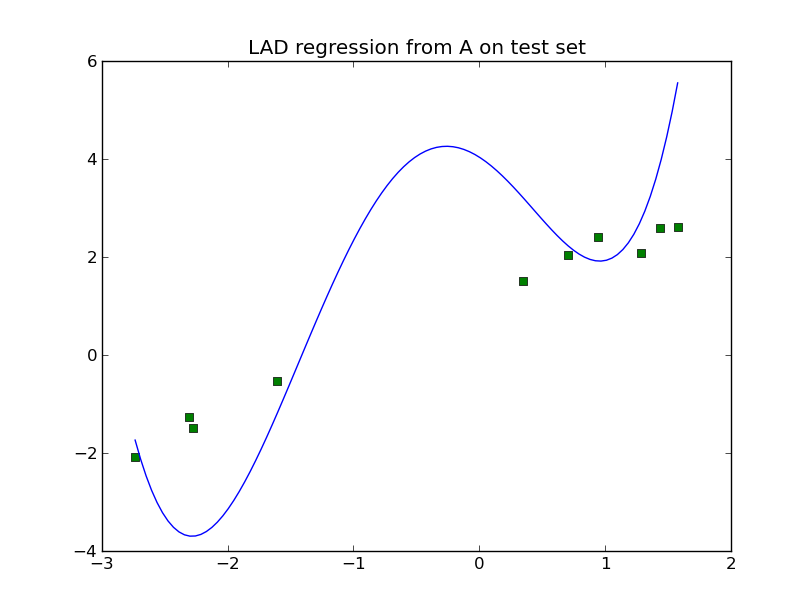
\includegraphics[scale=0.17]{./img/LAD_test_A.png}
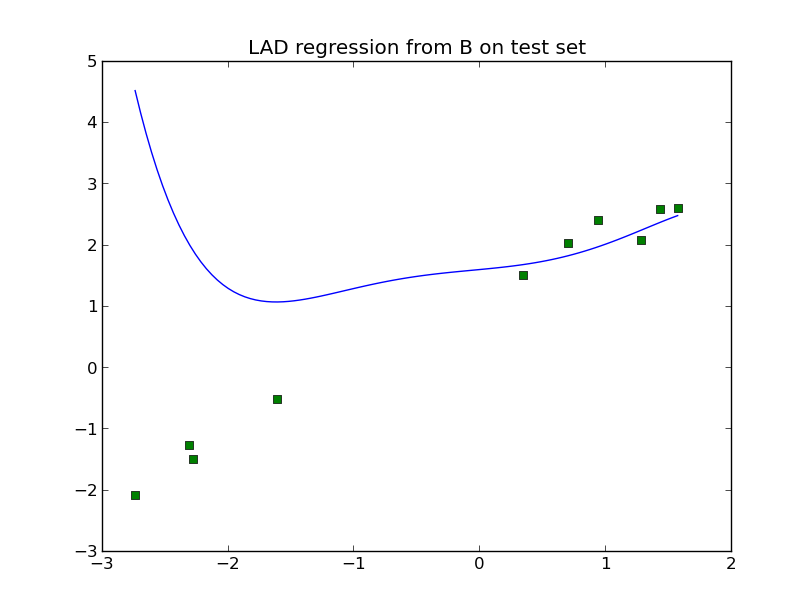
\includegraphics[scale=0.17]{./img/LAD_B_test.png}
\captionof{figure}{Final LAD models ($order=5$) from $train_A$ and $train_B$'s fit on the test set.} 
\endgroup

Final test errors for both selected models are $SAE_{test}^{(A)} = 13$, $SAE_{test}^{(B)} = 16$. We can see on figure 7 that the model from $train_A$ has less extreme test errors, whereas the model from $train_B$ predicts very well a cluster of data while having catastrophic fit on another cluster (small x). However they have comparable test error, as LAD does not penalize for extreme errors (as OLS does), as is discussed in 3.

\subsection{LASSO}

We implement the LASSO regularization of OLS, using gradient descent. Same process as in 1. is replicated.

\begin{table}[H]
\caption{Some $(M, \lambda)$ combinations validation errors for LASSO ($order = 5$). Minimum SSE for each training set in blue.}
\centering
\begin{tabular}{llrr}
\toprule
Training set & $\lambda$ & $SSE_{val}$ \\
\midrule

A & $10^{-4}$ &  5.8\\
A & $1$ & \textcolor{blue}{3.4}\\
A & $10^3$ & 24\\
B & $10^{-2}$ & 139\\
B & $1$ & 94\\
B & $10^4$ & \textcolor{blue}{25}\\
\bottomrule
\end{tabular}
\end{table}


Due to its preference to models with few non-zero parameters, LASSO on $train_B$ drives all parameters close to 0 with $\lambda=10^{3}$ or more. The selected model (minimum validation error), with $\lambda=10^{4}$, has all its coefficients of order $10^{-4}$ or less, and is almost a flat line.
\vspace{.1 in}

\begingroup
\centering
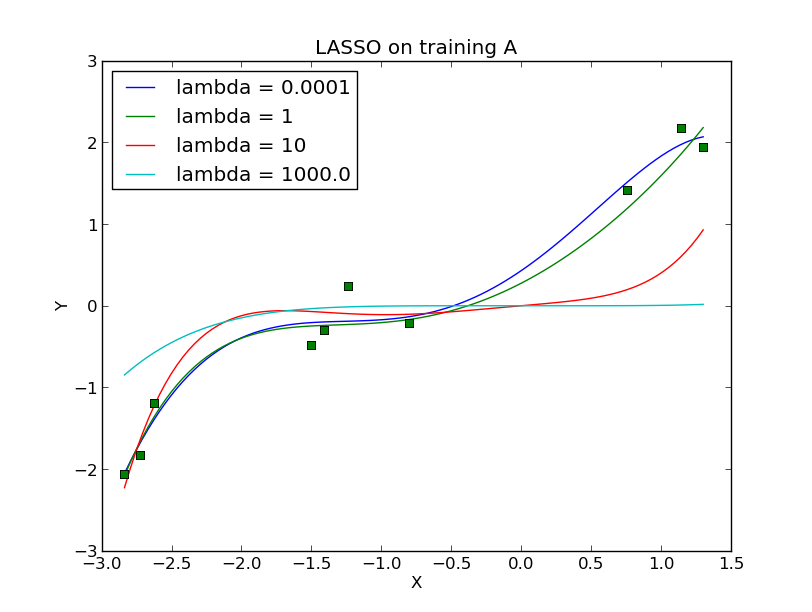
\includegraphics[scale=0.17]{./img/LASSO_A.png}
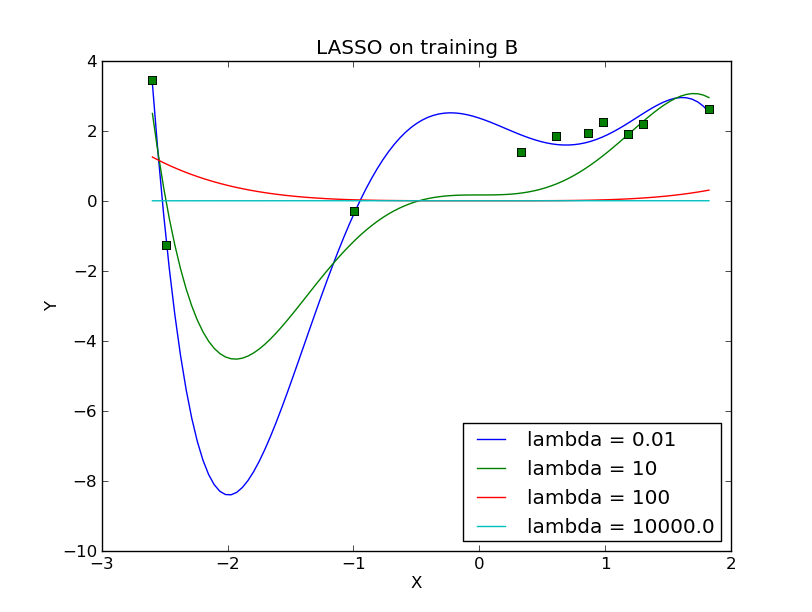
\includegraphics[scale=0.17]{./img/LASSO_B.png}
\captionof{figure}{Training fit for LASSO ($order=5$) with different $\lambda$ for $train_A$ (left) and $train_B$ (right).} 
\endgroup
\vspace{0.2 in}

\begingroup
\centering
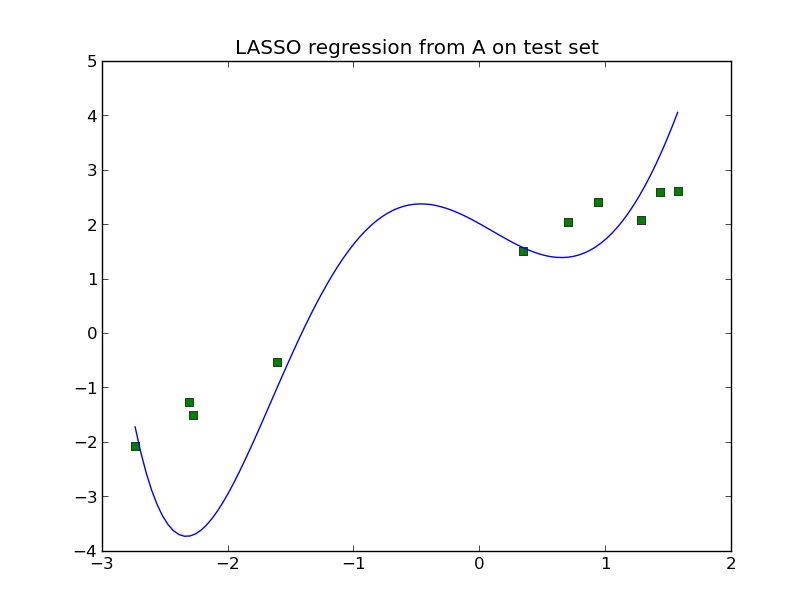
\includegraphics[scale=0.17]{./img/LASSO_test_A.png}
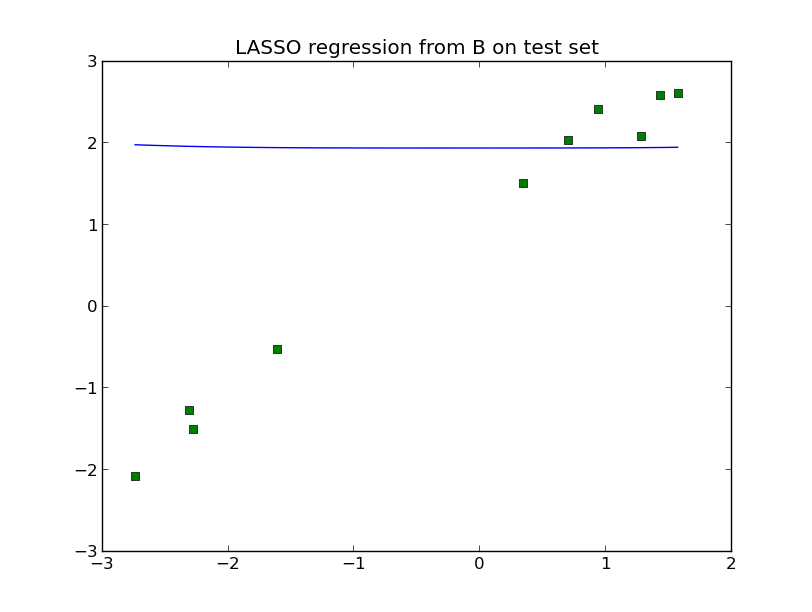
\includegraphics[scale=0.17]{./img/LASSO_test_B.png}
\captionof{figure}{Final LASSO models ($order=5$) from $train_A$ and $train_B$'s fit on the test set.} 
\endgroup

Final test errors for both selected models are $SSE_{test}^{(A)} = 6.02$, $SSE_{test}^{(B)} = 15.6$.

\subsection{Difference of approach}

LAD changes from ridge regression in the objective function we try to minimize, i.e. the error function we put on our fit and predictions. LAD is notably derived from using the absolute value loss function $L(p, a) = \left| p - a \right|$ in a prediction problem. Unlike least squares, this loss function does not penalize more heavily incremental regression error when the predicted value is far from the observed value (linear error). We might want to use LAD when we want every observation to be treated equally in the model fit (whereas LS gives greater weight to observations predicted poorly), to avoid strong effect from outliers. The training set $train_B$ gives a good example of a case where this is problematic for the linear fit (robust regression also provides a solution to this issue). LAD has notably been used in economics and biomedical studies.\\

Lasso has the advantage of bringing less significant parameters to 0, which is a useful for feature selection. This characteristic of Lasso to prefer fewer nonzero parameters make it a privileged solution for application like compressed sensing (signal processing).
%----------------------------------------------------------------------------------------
%	Appendix
%----------------------------------------------------------------------------------------

\appendix
\section{Figures}



%----------------------------------------------------------------------------------------

%\end{multicols}

\end{document}
